% !Mode:: "TeX:UTF-8"

\chapter{}
\textbf{
6.考虑到地震救灾场景,$n$个伤员需要被尽快总往医院。在这个地区有$k$ 所医院,这$n$个人中每个人需要被送到距离他们目前的地点半小时车程以内的医院(因此不同的人将对医院有不同的选择,依赖于他们当前所在的地方)。同时,人们不想由于太多的病人送来而使得任何一个医院超负荷。医护人员通过移动电话联系,他们想共同解决是否可以为每个受伤的人选择一所医院,这种选择方式要求医院负荷是均衡的,即每个医院至多接受$\lceil n/k\rceil$ 的人。给出一个多项式时间的算法,它以关于这些人所在位置的给定信息作为输入并且确定这是不可能的。
}

我们将伤员($w_i$)和医院($h_j$)表示成点,根据题目条件,加上源点$s$ 和汇点$t$可以构成Fig~\ref{q6_1}。
\begin{figure}[H]
  \centering
  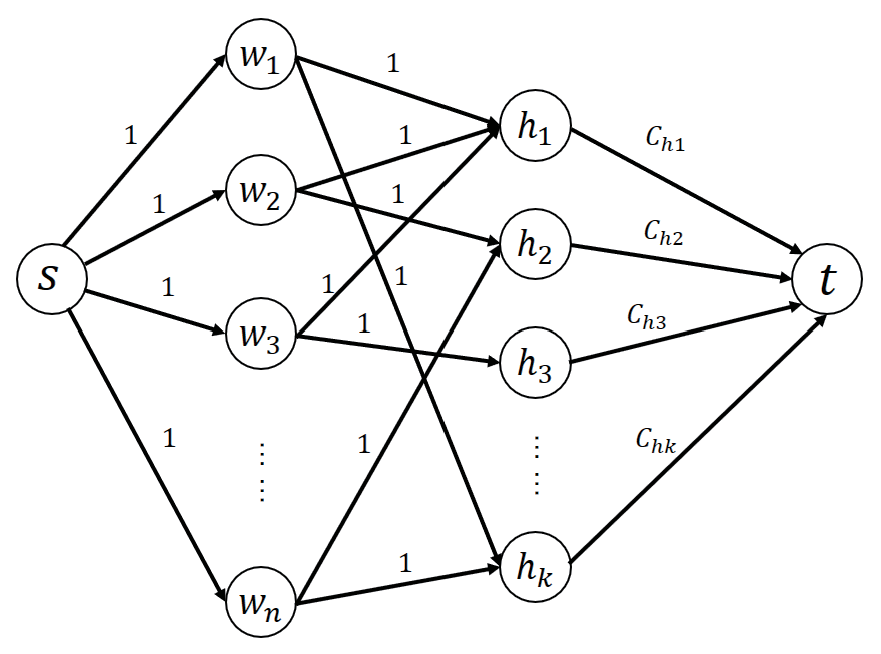
\includegraphics[width=0.7\textwidth]{figures/4.eps}\\
  \caption{Instance}\label{q6_1}
\end{figure}
图中$C_{hi}$ $(1\leq i\leq k)$ 表示各个医院的最大容量。因此只要执行最大流算法,就可以计算出结果。最大流算法的时间复杂度是多项式时间的。